% Options for packages loaded elsewhere
\PassOptionsToPackage{unicode}{hyperref}
\PassOptionsToPackage{hyphens}{url}
\PassOptionsToPackage{dvipsnames,svgnames,x11names}{xcolor}
%
\documentclass[
  letterpaper,
  DIV=11,
  numbers=noendperiod]{scrreprt}

\usepackage{amsmath,amssymb}
\usepackage{iftex}
\ifPDFTeX
  \usepackage[T1]{fontenc}
  \usepackage[utf8]{inputenc}
  \usepackage{textcomp} % provide euro and other symbols
\else % if luatex or xetex
  \usepackage{unicode-math}
  \defaultfontfeatures{Scale=MatchLowercase}
  \defaultfontfeatures[\rmfamily]{Ligatures=TeX,Scale=1}
\fi
\usepackage{lmodern}
\ifPDFTeX\else  
    % xetex/luatex font selection
\fi
% Use upquote if available, for straight quotes in verbatim environments
\IfFileExists{upquote.sty}{\usepackage{upquote}}{}
\IfFileExists{microtype.sty}{% use microtype if available
  \usepackage[]{microtype}
  \UseMicrotypeSet[protrusion]{basicmath} % disable protrusion for tt fonts
}{}
\makeatletter
\@ifundefined{KOMAClassName}{% if non-KOMA class
  \IfFileExists{parskip.sty}{%
    \usepackage{parskip}
  }{% else
    \setlength{\parindent}{0pt}
    \setlength{\parskip}{6pt plus 2pt minus 1pt}}
}{% if KOMA class
  \KOMAoptions{parskip=half}}
\makeatother
\usepackage{xcolor}
\setlength{\emergencystretch}{3em} % prevent overfull lines
\setcounter{secnumdepth}{5}
% Make \paragraph and \subparagraph free-standing
\makeatletter
\ifx\paragraph\undefined\else
  \let\oldparagraph\paragraph
  \renewcommand{\paragraph}{
    \@ifstar
      \xxxParagraphStar
      \xxxParagraphNoStar
  }
  \newcommand{\xxxParagraphStar}[1]{\oldparagraph*{#1}\mbox{}}
  \newcommand{\xxxParagraphNoStar}[1]{\oldparagraph{#1}\mbox{}}
\fi
\ifx\subparagraph\undefined\else
  \let\oldsubparagraph\subparagraph
  \renewcommand{\subparagraph}{
    \@ifstar
      \xxxSubParagraphStar
      \xxxSubParagraphNoStar
  }
  \newcommand{\xxxSubParagraphStar}[1]{\oldsubparagraph*{#1}\mbox{}}
  \newcommand{\xxxSubParagraphNoStar}[1]{\oldsubparagraph{#1}\mbox{}}
\fi
\makeatother


\providecommand{\tightlist}{%
  \setlength{\itemsep}{0pt}\setlength{\parskip}{0pt}}\usepackage{longtable,booktabs,array}
\usepackage{calc} % for calculating minipage widths
% Correct order of tables after \paragraph or \subparagraph
\usepackage{etoolbox}
\makeatletter
\patchcmd\longtable{\par}{\if@noskipsec\mbox{}\fi\par}{}{}
\makeatother
% Allow footnotes in longtable head/foot
\IfFileExists{footnotehyper.sty}{\usepackage{footnotehyper}}{\usepackage{footnote}}
\makesavenoteenv{longtable}
\usepackage{graphicx}
\makeatletter
\newsavebox\pandoc@box
\newcommand*\pandocbounded[1]{% scales image to fit in text height/width
  \sbox\pandoc@box{#1}%
  \Gscale@div\@tempa{\textheight}{\dimexpr\ht\pandoc@box+\dp\pandoc@box\relax}%
  \Gscale@div\@tempb{\linewidth}{\wd\pandoc@box}%
  \ifdim\@tempb\p@<\@tempa\p@\let\@tempa\@tempb\fi% select the smaller of both
  \ifdim\@tempa\p@<\p@\scalebox{\@tempa}{\usebox\pandoc@box}%
  \else\usebox{\pandoc@box}%
  \fi%
}
% Set default figure placement to htbp
\def\fps@figure{htbp}
\makeatother
% definitions for citeproc citations
\NewDocumentCommand\citeproctext{}{}
\NewDocumentCommand\citeproc{mm}{%
  \begingroup\def\citeproctext{#2}\cite{#1}\endgroup}
\makeatletter
 % allow citations to break across lines
 \let\@cite@ofmt\@firstofone
 % avoid brackets around text for \cite:
 \def\@biblabel#1{}
 \def\@cite#1#2{{#1\if@tempswa , #2\fi}}
\makeatother
\newlength{\cslhangindent}
\setlength{\cslhangindent}{1.5em}
\newlength{\csllabelwidth}
\setlength{\csllabelwidth}{3em}
\newenvironment{CSLReferences}[2] % #1 hanging-indent, #2 entry-spacing
 {\begin{list}{}{%
  \setlength{\itemindent}{0pt}
  \setlength{\leftmargin}{0pt}
  \setlength{\parsep}{0pt}
  % turn on hanging indent if param 1 is 1
  \ifodd #1
   \setlength{\leftmargin}{\cslhangindent}
   \setlength{\itemindent}{-1\cslhangindent}
  \fi
  % set entry spacing
  \setlength{\itemsep}{#2\baselineskip}}}
 {\end{list}}
\usepackage{calc}
\newcommand{\CSLBlock}[1]{\hfill\break\parbox[t]{\linewidth}{\strut\ignorespaces#1\strut}}
\newcommand{\CSLLeftMargin}[1]{\parbox[t]{\csllabelwidth}{\strut#1\strut}}
\newcommand{\CSLRightInline}[1]{\parbox[t]{\linewidth - \csllabelwidth}{\strut#1\strut}}
\newcommand{\CSLIndent}[1]{\hspace{\cslhangindent}#1}

\usepackage{booktabs}
\usepackage{longtable}
\usepackage{array}
\usepackage{multirow}
\usepackage{wrapfig}
\usepackage{float}
\usepackage{colortbl}
\usepackage{pdflscape}
\usepackage{tabu}
\usepackage{threeparttable}
\usepackage{threeparttablex}
\usepackage[normalem]{ulem}
\usepackage{makecell}
\usepackage{xcolor}
\KOMAoption{captions}{tableheading}
\makeatletter
\@ifpackageloaded{bookmark}{}{\usepackage{bookmark}}
\makeatother
\makeatletter
\@ifpackageloaded{caption}{}{\usepackage{caption}}
\AtBeginDocument{%
\ifdefined\contentsname
  \renewcommand*\contentsname{Table of contents}
\else
  \newcommand\contentsname{Table of contents}
\fi
\ifdefined\listfigurename
  \renewcommand*\listfigurename{List of Figures}
\else
  \newcommand\listfigurename{List of Figures}
\fi
\ifdefined\listtablename
  \renewcommand*\listtablename{List of Tables}
\else
  \newcommand\listtablename{List of Tables}
\fi
\ifdefined\figurename
  \renewcommand*\figurename{Figure}
\else
  \newcommand\figurename{Figure}
\fi
\ifdefined\tablename
  \renewcommand*\tablename{Table}
\else
  \newcommand\tablename{Table}
\fi
}
\@ifpackageloaded{float}{}{\usepackage{float}}
\floatstyle{ruled}
\@ifundefined{c@chapter}{\newfloat{codelisting}{h}{lop}}{\newfloat{codelisting}{h}{lop}[chapter]}
\floatname{codelisting}{Listing}
\newcommand*\listoflistings{\listof{codelisting}{List of Listings}}
\makeatother
\makeatletter
\makeatother
\makeatletter
\@ifpackageloaded{caption}{}{\usepackage{caption}}
\@ifpackageloaded{subcaption}{}{\usepackage{subcaption}}
\makeatother

\usepackage{bookmark}

\IfFileExists{xurl.sty}{\usepackage{xurl}}{} % add URL line breaks if available
\urlstyle{same} % disable monospaced font for URLs
\hypersetup{
  pdftitle={Evaluation of Office Vs. Non-Office Fall Injuries},
  pdfauthor={Ty Hansen},
  colorlinks=true,
  linkcolor={blue},
  filecolor={Maroon},
  citecolor={Blue},
  urlcolor={Blue},
  pdfcreator={LaTeX via pandoc}}


\title{Evaluation of Office Vs. Non-Office Fall Injuries}
\author{Ty Hansen}
\date{}

\begin{document}
\maketitle

\renewcommand*\contentsname{Table of contents}
{
\hypersetup{linkcolor=}
\setcounter{tocdepth}{2}
\tableofcontents
}

\bookmarksetup{startatroot}

\chapter{Executive Summary}\label{executive-summary}

\section{Overview}\label{overview}

This report evaluates whether office workers at ABC Corp face greater
fall injury risk than non office workers, and whether stronger office
safety policies are warranted. The analysis was prompted by a concern
raised by our safety officer following a recent article suggesting
office workers are more prone to fall injuries than workers in other
environments. Using data from the BLS Survey of Occupational Injuries
and Illnesses (SOII) ({``{IIF} Databases : U.s. Bureau of Labor
Statistics''} 2024), overall injury rates and same level fall rates were
compared across office and non office industries.

\section{Key Findings}\label{key-findings}

Office industries averaged 6.5 same level fall cases per 10,000 FTE
workers, compared to 15.7 for non office industries, a statistically
significant difference (t(3.5) = -3.64, p = 0.027). Overall injury rates
follow the same pattern. Office industries reported total recordable
case (TRC) rates well below non office industries and the private
industry average. The data does not support the claim that office
workers are at greater fall risk than non office workers.

\section{Recommendations}\label{recommendations}

Based on these findings, it is recommended that the safety officer
direct resources toward the company's industrial and manufacturing
operations, where injury risk is substantially higher. A major policy
change for office workers is not justified by the evidence. Basic office
safety precautions, such as cable management, adequate lighting, and non
slip flooring, remain worthwhile but do not require significant new
investment.

\section{Next Steps}\label{next-steps}

Future analysis should examine whether specific office roles, such as
facilities or mailroom staff, carry elevated injury risk compared to
fully desk based employees. If the company's workforce shifts toward
hybrid and remote work arrangements, it will be worth investigating how
injury patterns change over time. Occupation level data from the SOII
would allow for a more in depth analysis than the industry level
comparison presented here.

\bookmarksetup{startatroot}

\chapter{Introduction}\label{introduction}

ABC Corp operates across both office and industrial environments, and
ensuring the safety of all employees is a shared priority. This report
was prepared in response to a concern raised by our safety officer
regarding fall injury risk among office workers. Specifically, a recent
article suggested that office workers are more likely to be injured
through falls than workers in other environments, raising the question
of whether ABC Corp should implement stronger safety policies for office
staff. Using data from the BLS (Bureau of Labor Statistics) Survey of
Occupational Injuries and Illnesses (SOII) ({``{IIF} Databases : U.s.
Bureau of Labor Statistics''} 2024), this report compares overall injury
rates and same-level fall rates across office and non-office industries
to evaluate this claim. Risk is assessed on two factors: the probability
of injury occurring and the severity of that injury as measured by days
away from work (DAFW).

\emph{Potential Risk} ({``Slips, {Trips}, and {Falls}: {Workplace
Injuries} in {New York}''} 2023)
\pandocbounded{\includegraphics[keepaspectratio]{Slips-Trips-and-Falls-Workplace-Injuries-in-New-York.jpg.webp}}
The report proceeds as follows. The Data Documentation section
(Appendix~\ref{sec-data-doc}) describes the data source, key variables,
and industry classifications used. The Results section
(Chapter~\ref{sec-results}) presents descriptive statistics by industry,
a comparison of same-level fall rates between office and non-office
industries, and the results of a two-sample Welch t-test. The Conclusion
(Chapter~\ref{sec-conclusion}) summarizes the findings and provides a
recommendation to the safety officer on whether additional office safety
policies are justified.

\bookmarksetup{startatroot}

\chapter{Data Documentation and Methodology}\label{sec-data-doc}

\section{Data Documentation}\label{data-documentation}

The U.S. Bureau of Labor Statistics (BLS), in cooperation with state
labor agencies, collects and publishes the data used in this report
({``{IIF} Databases : U.s. Bureau of Labor Statistics''} 2024). The BLS
collects this data to track nonfatal workplace injuries and illnesses at
the national level and to help employers, policymakers, and researchers
identify safety trends and allocate resources appropriately. The data
covers work-related injuries, illnesses, and fatalities across
privateindustry and state and local government. This includes rates by
industry, injury type, event or exposure, and severity as measured by
days away from work. The BLS has collected workplace injury and illness
data annually since 1972. The most recent summary data used in this
report cover reference year 2024, with biennial case and demographic
detail available for the 2023--2024 period. Data is collected from
employers across all 50 states through a sample of approximately 200,000
establishments, providing nationally representative estimates. Employers
are legally required under OSHA regulations to log all recordable work
related injuries and illnesses on OSHA Form 300 and to submit summary
information annually. The BLS uses these records, collected through the
Survey of Occupational Injuries and Illnesses (SOII), to produce
national and state level estimates. The data is organized into summary
tables reporting injury and illness rates by detailed industry, and case
and demographic tables reporting rates by event type, worker
characteristics, and other case circumstances. Data used in this
analysis come from the BLS Survey of Occupational Injuries and Illnesses
(SOII), accessed through the Injuries, Illnesses, and Fatalities (IIF)
database ({``{IIF} Databases : U.s. Bureau of Labor Statistics''} 2024).
Two tables are used: Table 1 reports total recordable case (TRC) rates,
defined as the count of all recordable workplace injuries and illnesses
per 100 full-time equivalent (FTE) workers by industry for 2024. Table
R75 reports days away from work (DAFW) fall rates---injuries serious
enough to require at least one day off work---per 10,000 FTE workers by
industry division for 2023--2024.

Industries are classified using the North American Industry
Classification System (NAICS) and are further grouped as office or
non-office based on whether work is primarily desk-based.

Incidence rates in summary tables are expressed per 100 full-time
equivalent (FTE) workers, while rates in the detailed case and
demographic tables are expressed per 10,000 FTE workers. Cells based on
fewer than 15 cases are suppressed and left blank to protect
confidentiality and ensure reliability.

The BLS runs consistency checks on all submitted data and publishes
error estimates alongside its tables. A known limitation of the SOII is
underreporting; some employers may fail to record or report all
qualifying injuries and illnesses. While the magnitude of underreporting
is difficult to quantify, BLS-funded research suggests it is a real
concern. However, there is no strong reason to believe underreporting
differs between office and non-office industries in a way that would
affect the conclusions of this report.

The data is produced by the U.S. federal government and is in the public
domain, available at no cost through the BLS IIF database ({``{IIF}
Databases : U.s. Bureau of Labor Statistics''} 2024).

\section{Methodology}\label{methodology}

The primary analysis in this report compares same level fall rates
between office and non office industries. Days away from work are used
as a benchmark for injury severity, and a two sample t-test is used to
assess whether differences between groups are statistically significant.

Data is recorded using OSHA Forms 300, 300A, and 301. The BLS uses its
Occupational Injury and Illness Classification System (OIICS) to code
case circumstances, and industries and occupations are classified using
NAICS and SOC, respectively.

\bookmarksetup{startatroot}

\chapter{Results}\label{sec-results}

\section{Descriptive Statistics}\label{descriptive-statistics}

Table~\ref{tbl-summary} shows overall injury rates and same-level fall
rates for each industry sector. Office industries have noticeably lower
rates across both measures compared to non-office industries.

\begin{longtable}[t]{lccc}

\caption{\label{tbl-summary}TRC rates (per 100 FTE) and same-level fall
DAFW rates (per 10,000 FTE) by industry. Source: BLS SOII ({``{IIF}
Databases : U.s. Bureau of Labor Statistics''} 2024).}

\tabularnewline

\toprule
Industry & Category & TRC Rate & Same-Level Fall DAFW Rate\\
\midrule
\cellcolor{lightblue}{Finance and Insurance} & \cellcolor{lightblue}{Office} & \cellcolor{lightblue}{0.3} & \cellcolor{lightblue}{5.4}\\
\cellcolor{lightblue}{Information} & \cellcolor{lightblue}{Office} & \cellcolor{lightblue}{0.7} & \cellcolor{lightblue}{7.9}\\
\cellcolor{lightblue}{Professional \& Business Services} & \cellcolor{lightblue}{Office} & \cellcolor{lightblue}{1.0} & \cellcolor{lightblue}{6.2}\\
\cellcolor{salmon}{Construction} & \cellcolor{salmon}{Non-Office} & \cellcolor{salmon}{2.2} & \cellcolor{salmon}{11.0}\\
\cellcolor{salmon}{Manufacturing} & \cellcolor{salmon}{Non-Office} & \cellcolor{salmon}{2.7} & \cellcolor{salmon}{12.1}\\
\addlinespace
\cellcolor{salmon}{Natural Resources \& Mining} & \cellcolor{salmon}{Non-Office} & \cellcolor{salmon}{2.8} & \cellcolor{salmon}{19.6}\\
\cellcolor{salmon}{Trade, Transportation \& Utilities} & \cellcolor{salmon}{Non-Office} & \cellcolor{salmon}{3.1} & \cellcolor{salmon}{20.2}\\
\bottomrule

\end{longtable}

\section{Analysis}\label{analysis}

To formally evaluate the safety officer's claim, same-level fall DAFW
rates were compared between office and non-office industries using a
two-sample Welch t-test. This test is appropriate here because we are
comparing the means of two independent groups and do not assume equal
variances between them. The goal is to determine whether any observed
difference in fall rates between office and non-office industries is
statistically significant or likely due to chance.

\textbf{Ho:} Mean same-level fall rate is equal between office and
non-office industries.\\
\textbf{Ha:} Mean same-level fall rate differs between the two groups.

\begin{longtable}[t]{llcccccc}

\caption{\label{tbl-ttest}Two-sample t-test results for same-level fall
DAFW rates (per 10,000 FTE) by group.}

\tabularnewline

\toprule
 & Group & Mean & SD & t & df & p-value & 95\% CI\\
\midrule
t & Office & 6.5 & 1.3 & -3.64 & 3.5 & 0.027 & {}[-16.64, -1.81]\\
 & Non-Office & 15.7 & 4.8 & NA & NA & NA & NA\\
\bottomrule

\end{longtable}

The results show a statistically significant difference in same-level
fall rates between office and non-office industries (t(3.5) = -3.64, p =
0.027, 95\% CI {[}-16.64, -1.81{]}). Office industries averaged 6.5
same-level fall cases per 10,000 FTE workers, compared to 15.7 for
non-office industries. These findings do not support the safety
officer's claim --- office workers experience significantly fewer
same-level fall injuries than their non-office counterparts.

\begin{figure}

\centering{

\pandocbounded{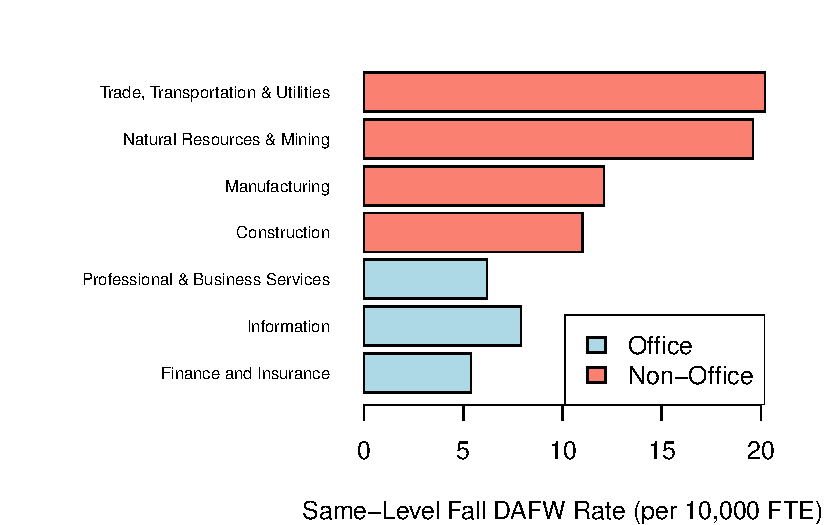
\includegraphics[keepaspectratio]{results_files/figure-pdf/fig-falls-1.pdf}}

}

\caption{\label{fig-falls}Same-level fall DAFW rates by industry (per
10,000 FTE). Source: BLS SOII Table R75 ({``{IIF} Databases : U.s.
Bureau of Labor Statistics''} 2024).}

\end{figure}%

\bookmarksetup{startatroot}

\chapter{Summary}\label{sec-conclusion}

\textbf{Key finding:} Office workers experience significantly fewer
same-level fall injuries than non-office workers. This report does not
recommend a major policy overhaul for office staff.

Office industries averaged 6.5 same-level fall cases per 10,000 FTE
workers, compared to 15.7 for non-office industries (t(3.5) = -3.64, p =
0.027, 95\% CI {[}-16.64, -1.81{]}). Overall injury rates follow the
same pattern, with office industries reporting TRC rates well below
non-office industries and the private industry average. These results
are consistent with what one would expect given the physical demands of
non-office work, and they contradict the claim in the article that
prompted this investigation.

There are several limitations to consider. The t-test was conducted on
only seven industry divisions --- three office and four non-office ---
resulting in low statistical power. While the result is statistically
significant, the small number of industries means findings should be
interpreted with some caution. The SOII data also rely on
employer-reported injuries, and underreporting is a known limitation,
though there is no strong reason to believe underreporting differs
systematically between office and non-office settings in a way that
would reverse these findings. It is also worth noting that classifying
industries as simply office or non-office is a simplification --- many
industries, including ABC Corp itself, contain both types of workers.
Future analysis using occupation-level data would allow for a more
precise comparison.

It is recommended that ABC Corp's safety officer focus resources on the
company's industrial and manufacturing operations, where injury risk is
substantially higher. This does not mean office safety should be
neglected --- basic precautions such as cable management, appropriate
lighting, and non-slip flooring remain worthwhile. However, a major
policy change for office workers is not justified by the evidence. Going
forward, it may be worth examining whether specific office roles such as
facilities or mailroom staff carry elevated risk compared to fully
desk-based employees, and how the shift toward hybrid work might affect
injury patterns over time.

\bookmarksetup{startatroot}

\chapter*{References}\label{references}
\addcontentsline{toc}{chapter}{References}

\markboth{References}{References}

\phantomsection\label{refs}
\begin{CSLReferences}{1}{0}
\bibitem[\citeproctext]{ref-IIFDatabasesUS}
{``{IIF} Databases : U.s. Bureau of Labor Statistics.''} 2024. January
1, 2024. \url{https://www.bls.gov/iif/data.htm}.

\bibitem[\citeproctext]{ref-SlipsTripsFalls2023}
{``Slips, {Trips}, and {Falls}: {Workplace Injuries} in {New York}.''}
2023. October 18, 2023. \url{https://nylaw.net/slip-trips-and-falls/}.

\end{CSLReferences}

\cleardoublepage
\phantomsection
\addcontentsline{toc}{part}{Appendices}
\appendix

\chapter{Data Documentation and Methodology}\label{sec-data-doc}

\section{Data Documentation}\label{data-documentation-1}

The U.S. Bureau of Labor Statistics (BLS), in cooperation with state
labor agencies, collects and publishes the data used in this report
({``{IIF} Databases : U.s. Bureau of Labor Statistics''} 2024). The BLS
collects this data to track nonfatal workplace injuries and illnesses at
the national level and to help employers, policymakers, and researchers
identify safety trends and allocate resources appropriately. The data
covers work-related injuries, illnesses, and fatalities across
privateindustry and state and local government. This includes rates by
industry, injury type, event or exposure, and severity as measured by
days away from work. The BLS has collected workplace injury and illness
data annually since 1972. The most recent summary data used in this
report cover reference year 2024, with biennial case and demographic
detail available for the 2023--2024 period. Data is collected from
employers across all 50 states through a sample of approximately 200,000
establishments, providing nationally representative estimates. Employers
are legally required under OSHA regulations to log all recordable work
related injuries and illnesses on OSHA Form 300 and to submit summary
information annually. The BLS uses these records, collected through the
Survey of Occupational Injuries and Illnesses (SOII), to produce
national and state level estimates. The data is organized into summary
tables reporting injury and illness rates by detailed industry, and case
and demographic tables reporting rates by event type, worker
characteristics, and other case circumstances. Data used in this
analysis come from the BLS Survey of Occupational Injuries and Illnesses
(SOII), accessed through the Injuries, Illnesses, and Fatalities (IIF)
database ({``{IIF} Databases : U.s. Bureau of Labor Statistics''} 2024).
Two tables are used: Table 1 reports total recordable case (TRC) rates,
defined as the count of all recordable workplace injuries and illnesses
per 100 full-time equivalent (FTE) workers by industry for 2024. Table
R75 reports days away from work (DAFW) fall rates---injuries serious
enough to require at least one day off work---per 10,000 FTE workers by
industry division for 2023--2024.

Industries are classified using the North American Industry
Classification System (NAICS) and are further grouped as office or
non-office based on whether work is primarily desk-based.

Incidence rates in summary tables are expressed per 100 full-time
equivalent (FTE) workers, while rates in the detailed case and
demographic tables are expressed per 10,000 FTE workers. Cells based on
fewer than 15 cases are suppressed and left blank to protect
confidentiality and ensure reliability.

The BLS runs consistency checks on all submitted data and publishes
error estimates alongside its tables. A known limitation of the SOII is
underreporting; some employers may fail to record or report all
qualifying injuries and illnesses. While the magnitude of underreporting
is difficult to quantify, BLS-funded research suggests it is a real
concern. However, there is no strong reason to believe underreporting
differs between office and non-office industries in a way that would
affect the conclusions of this report.

The data is produced by the U.S. federal government and is in the public
domain, available at no cost through the BLS IIF database ({``{IIF}
Databases : U.s. Bureau of Labor Statistics''} 2024).

\section{Methodology}\label{methodology-1}

The primary analysis in this report compares same level fall rates
between office and non office industries. Days away from work are used
as a benchmark for injury severity, and a two sample t-test is used to
assess whether differences between groups are statistically significant.

Data is recorded using OSHA Forms 300, 300A, and 301. The BLS uses its
Occupational Injury and Illness Classification System (OIICS) to code
case circumstances, and industries and occupations are classified using
NAICS and SOC, respectively.

\chapter*{References}\label{references-1}
\addcontentsline{toc}{chapter}{References}

\markboth{References}{References}

\phantomsection\label{refs}
\begin{CSLReferences}{1}{0}
\bibitem[\citeproctext]{ref-IIFDatabasesUS}
{``{IIF} Databases : U.s. Bureau of Labor Statistics.''} 2024. January
1, 2024. \url{https://www.bls.gov/iif/data.htm}.

\bibitem[\citeproctext]{ref-SlipsTripsFalls2023}
{``Slips, {Trips}, and {Falls}: {Workplace Injuries} in {New York}.''}
2023. October 18, 2023. \url{https://nylaw.net/slip-trips-and-falls/}.

\end{CSLReferences}




\end{document}
